\chapter{Resultados}

O projeto está hospedado em um repositório público no GitHub, disponível em: 
\url{https://github.com/cardoso42/cartas-de-amor}

Foi possível gerar certificados digitais para o estabelecimento de conexão HTTPS com o site \url{https://cardoso42.site}, que está hospedado em uma instância da AWS. Isso garante a segurança na comunicação entre cliente e servidor, utilizando criptografia TLS.

A seguir, apresentamos uma captura de tela exemplificando o funcionamento do sistema:

\begin{figure}[H]
    \centering
    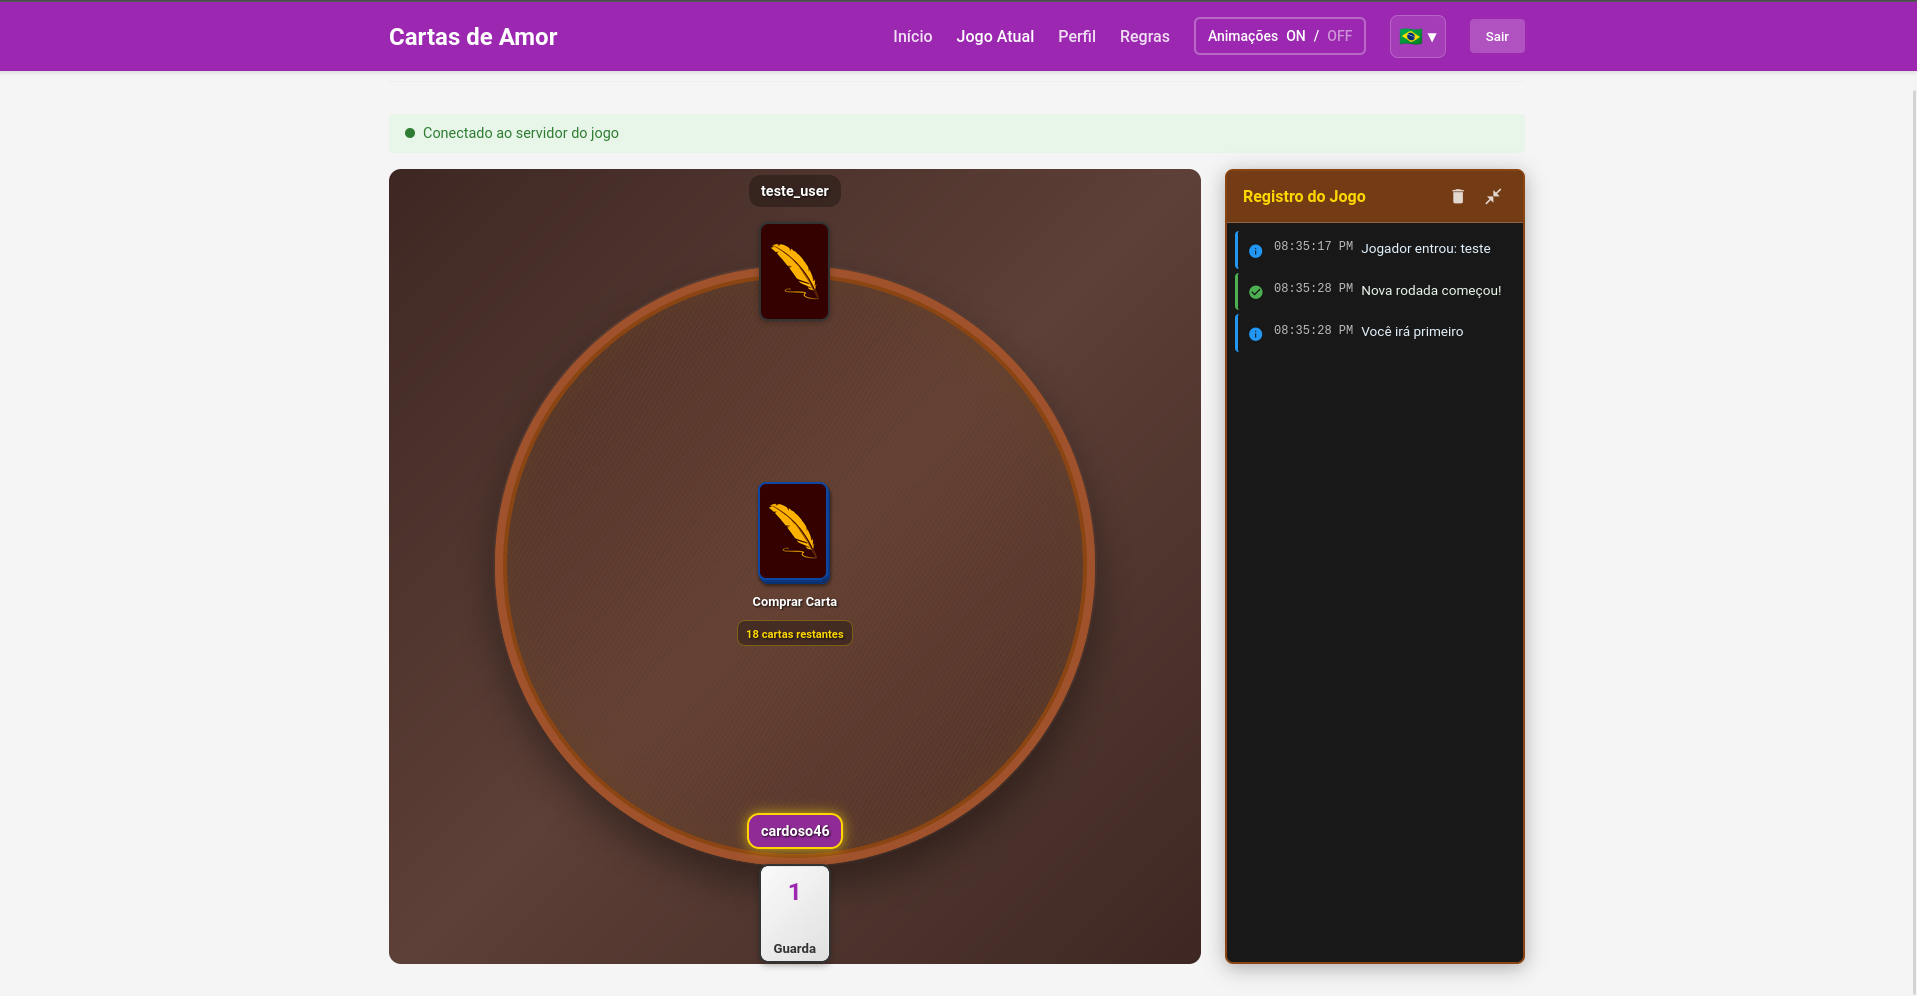
\includegraphics[width=0.8\textwidth]{screens/image.png}
    \caption{Exemplo de tela do sistema em funcionamento. Fonte: os autores}
    \label{fig:screen_example}
\end{figure}


